\documentclass[a4paper,ngerman,12pt]{scrartcl}

\usepackage[utf8]{inputenc}
%\usepackage[ansinew]{inputenc}

\usepackage[ngerman]{babel}

\usepackage{amsmath,amsthm,amssymb,stmaryrd,color,graphicx}
\usepackage{setspace}
\usepackage{bussproofs}
\usepackage{array}
\usepackage{comment}
\usepackage{wrapfig}

\usepackage{enumitem}

\usepackage{units}

\usepackage[protrusion=true,expansion=true]{microtype}

\usepackage{lmodern}

\usepackage{hyperref}
\usepackage{cleveref}

\newcommand{\RR}{\mathbb{R}}
\newcommand{\CC}{\mathbb{C}}
\newcommand{\ZZ}{\mathbb{Z}}
\newcommand{\NN}{\mathbb{N}}
\newcommand{\QQ}{\mathbb{Q}}

\setlength\parskip{\medskipamount}
\setlength\parindent{0pt}

\theoremstyle{definition}
\newtheorem{defn}{Definition}[]
\newtheorem{axiom}[defn]{Axiom}
\newtheorem{bsp}[defn]{Beispiel}

\theoremstyle{plain}
\newtheorem{prop}[defn]{Proposition}
\newtheorem{motto}[defn]{Motto}
\newtheorem{wunder}[defn]{Wunder}
\newtheorem{ueberlegung}[defn]{Überlegung}
\newtheorem{lemma}[defn]{Lemma}
\newtheorem{kor}[defn]{Korollar}
\newtheorem{hilfsaussage}[defn]{Hilfsaussage}
\newtheorem{satz}[defn]{Satz}
\newtheorem{frage}[defn]{Frage}

\theoremstyle{remark}
\newtheorem{bem}[defn]{Bemerkung}
\newtheorem{aufg}[defn]{Aufgabe}

\newtheorem*{antwort}{Antwort}

\newlength{\aufgabenskip}
\setlength{\aufgabenskip}{1.4em}
\newcounter{aufgabennummer}
\newenvironment{aufgabe}[1]{
	\addtocounter{aufgabennummer}{1}
	\textbf{Aufgabe \theaufgabennummer.} \emph{#1} \par
}{\vspace{\aufgabenskip}}

\clubpenalty=10000
\widowpenalty=10000
\displaywidowpenalty=10000

\setlength\unitlength{1cm}

\usepackage{tikz}

\RequirePackage{geometry}
\geometry{textwidth=16.0cm,textheight=24.5cm,footskip=1.5cm}

\begin{document}
	
\begin{picture}(0,0)
\put(0,-0.5){%
	
\includegraphics[scale=0.1]{logo-ifm}
}
\put(14.0,-3.5){%
	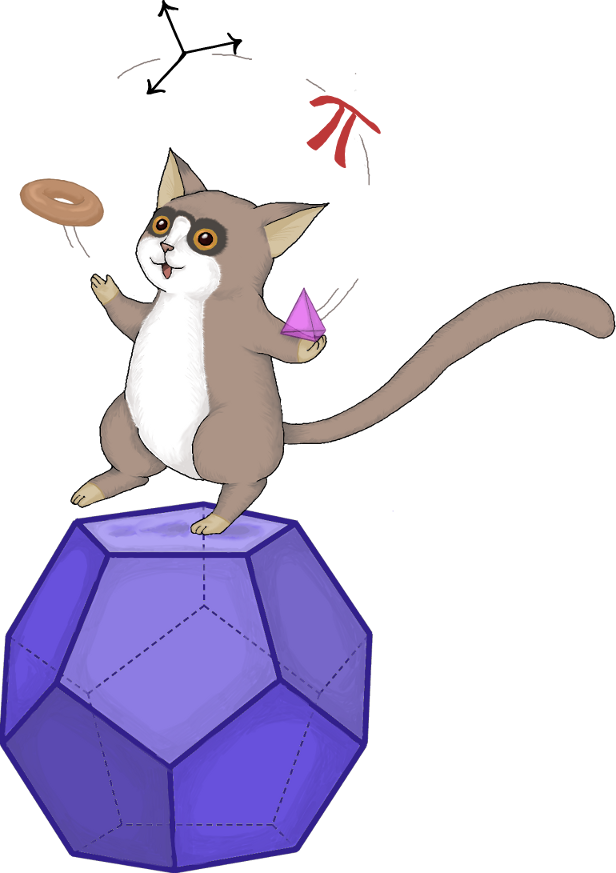
\includegraphics[scale=0.17]{cover}
}
\end{picture} 
	
\vspace{6em}

\section*{Unmöglichkeitsbeweise über Invarianten - Lösungshinweise}

Dieses Skript enthält Lösungs\emph{hinweise} zum letzten Korrespondenzbrief. Manchmal sind dies schon die kompletten Lösungen der Aufgaben, meistens sind es aber nur einige Hinweise, die dir dabei helfen sollen, auch die Aufgaben lösen zu können, bei denen du bisher nicht weiter gekommen bist. Wenn du noch weitere Fragen zu den Aufgaben hast, kannst du uns diese weiterhin gerne per E-Mail stellen.

Wenn du uns bereits deine eigenen Lösungsversuche geschickt hast (oder noch schicken wirst - das ist selbstverständlich immer noch möglich), dann versuchen wir natürlich auch dir mit unseren Korrekturen beim Verständnis der Aufgaben zu helfen. Es lohnt sich also uns deine Lösungen zu senden :-)

\begin{aufgabe}{}
	Für beide Fragen: Die Nachricht dreimal hintereinander schreiben
\end{aufgabe}

\begin{aufgabe}{}
	
\end{aufgabe}

\begin{aufgabe}{}
	$3$
\end{aufgabe}

\begin{aufgabe}{}
	172919 korrekt, Nachricht 1729
	
	422416 falsch
	
	939124 falsch
	
	314109 korrekt, Nachricht 3141
	
	739150 - falsch, hier muss der Fehler aber im hinteren Teil passiert sein (also in der Quersumme), da dieser größer als 36 (der Maximalwert) ist. Die Nachricht selbst ist also erhalten geblieben.
\end{aufgabe}

\begin{aufgabe}
	23836 korrekt
	
	99999 falsch
	
	47629 korrekt
	
	38425 falsch
\end{aufgabe}

\begin{aufgabe}{}
	Informationsrate $\frac{5}{4} = 1,25$
	
	Die Informationsrate wird besser, wenn man längere Nachrichtenworte verwendet.
\end{aufgabe}

\begin{aufgabe}{}

\end{aufgabe}

\end{document}